\chapter{Описание используемого подхода}
\label{chapter2} 

\section{Особенности ALE}
\subsection{Описание метода}

Как уже было изложено выше, ALE оценивает качество сборки при помощи следующей формулы:
$$P(A|R)=\frac{P_{placement}(R|A)P_{insert}(R|A)P_{depth}(R|A)P(A)}{Z}$$

\begin{figure}[h]
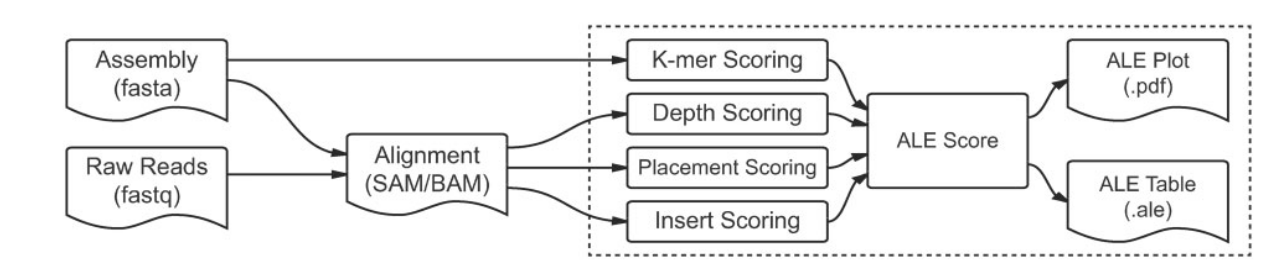
\includegraphics[width=\textwidth]{ale_scheme.png}
\caption{Общая схема работы ALE}
\label{fig:ALECommon}
\end{figure}

\subsubsection{Нормализационная константа $Z$}
$Z$ является константой, вычисляется как: 
$$Z = \sum_{A'}P(R|A')P(A')$$ Данную величину  вычисляют приближённо, поскольку явно её вычислить невозможно из-за слишком большого множества сборок $A'$ ($4^L$, где $L$ – длина сборки).

\subsubsection{Оценка сборки при отсутствии чтений}
$$P(A) = Z P_{kmer}(A)$$
$P_{kmer}(A) = \prod_{i \in K}f_{i}^{n_{i}}$, где $K$ – множество уникальных $k$-меров, $n_i$ – количество раз, когда $k$-мер $i$ встречается в текущем контиге в сборке. $f_i$ – частота появление $k$-мера $i$ в контиге: $f_i = n_i / \sum_{j \in K} n_j$.

\subsubsection{Корректность чтений}
$P_{placement}(R|A)$ -- оценивает насколько чтения соответствуют сборке, выражается следующим образом:$$P_{placement}(R|A)=\prod_{r_i \in R}P_{placement}(r_i|A)=$$
$$=\prod_{r_i \in R}P_{matches}(r_i|A)P_{orientation}(r_i|A)$$

$P_{matches}(r_i|A)$ оценивает, насколько содержимое чтения соответствует тому участку сборки, на который было произведено картирование данного чтения. Каждый нуклеотид $j$, считанный при помощи секвенатора имеет качество считывания $Q_j$, $Q_j\subseteq[0;1]$, тогда $P_{matches}(r_i|A) = \prod_{j \in r_i}P_{base_j|A}$, где $P_{base_j|A} = Q_j$ когда нуклеотид $j$ совпадает  со сборкой и $P_{base_j|A} = (1 - Q_j)/4$ в противном случае. Если в сборке встречается неизвестный нуклеотид $N$, то считаем, что $P_{base_j|A} = 1/4$
Если инструмент картирования сопоставил чтение более чем в одно место, ALE выбирает позицию, у которой $P_{placement}(R|A)$ наибольший.

$P_{orientation}(r_i|A)$ оценивает корректность ориентации в случае парных чтений. Величина вычисляется эмпирически.

\subsubsection{Расстояние между парными чтениями}
$P_{insert}(R|A)$ оценивает расстояние между парными чтениями, вычисляется как $P_{insert}(R|A)=\prod_{r_i \in R}P_{insert}(r_i|A)$. $P_{insert}(r_i|A) = Normal(L_i; \mu, \sigma^2)$ 

\subsection{Оценка глубины покрытия}

Рассмотрим более подробно вычисление $P_{depth}(R|A)$. Эта величина описывает, насколько глубина покрытия в каждой позиции, соответствует глубине, которую мы бы ожидали увидеть, если бы картирование производилось на эталонную сборку.
$$P_{depth}(R|A) = \prod_{i}P_{depth}(d_i|A)$$ $d_i$ – глубина в позиции $i$. Предполагается, что глубины распределены по Пуассону с центром, вычисленным из независимого гамма-распределения с центром в ожидаемой глубине в данной позиции и GC-контентом в качестве второго параметра. Рассмотрим это утверждение более подробно.

Сначала рассчитываются средние глубины для каждого из 100 множеств GC-контента: 0-1, 1-2 ... 99-100\%. Пусть $X_i$ – это средний GC-контент по всем чтениям, которые покрывают позицию $i$. $\mu_{depth}(X_i)$ – средняя глубина для того множества GC-контентов, которому соответствует $X_i$. Минимальное значение $\mu_{depth}(X_i)$ устанавливается равным 10. В итоге для каждой позиции $i$ в сборке оценка глубины будет производиться по следующей формуле:
$$P_{depth}(d_i|A, X_i)=\int_0^\infty Poisson(d_i, Y_i)Gamma(Y_i, max(10, \mu_{depth}(X_i), 1))dY_i =$$ $$=NegBinom(d_i, \mu_{depth}(X_i), 0.5)$$

Подытоживая вышесказанное, получаем, что глубины распределены по отрицательному биномиальному распределению $NB(r, p)$ с параметрами $r = \mu_{depth}(X_i)$ и $p = 0.5$.

\subsection{Проблема оценки глубины покрытия}
В ходе выполнения данной работы было выявлено, глубины покрытий распределены не по отрицательному биномиальному распределению.

Для того, чтобы убедиться в этом был для каждого из 100 множеств GC-контента было построено эмпирическое распределение глубин покрытий. В итоге получилась таблица $100\times maxdepth$, где $maxdepth$ -- это максимальное значение глубины покрытия позиции чтениями в данной сборке. 

\begin{figure}[H]
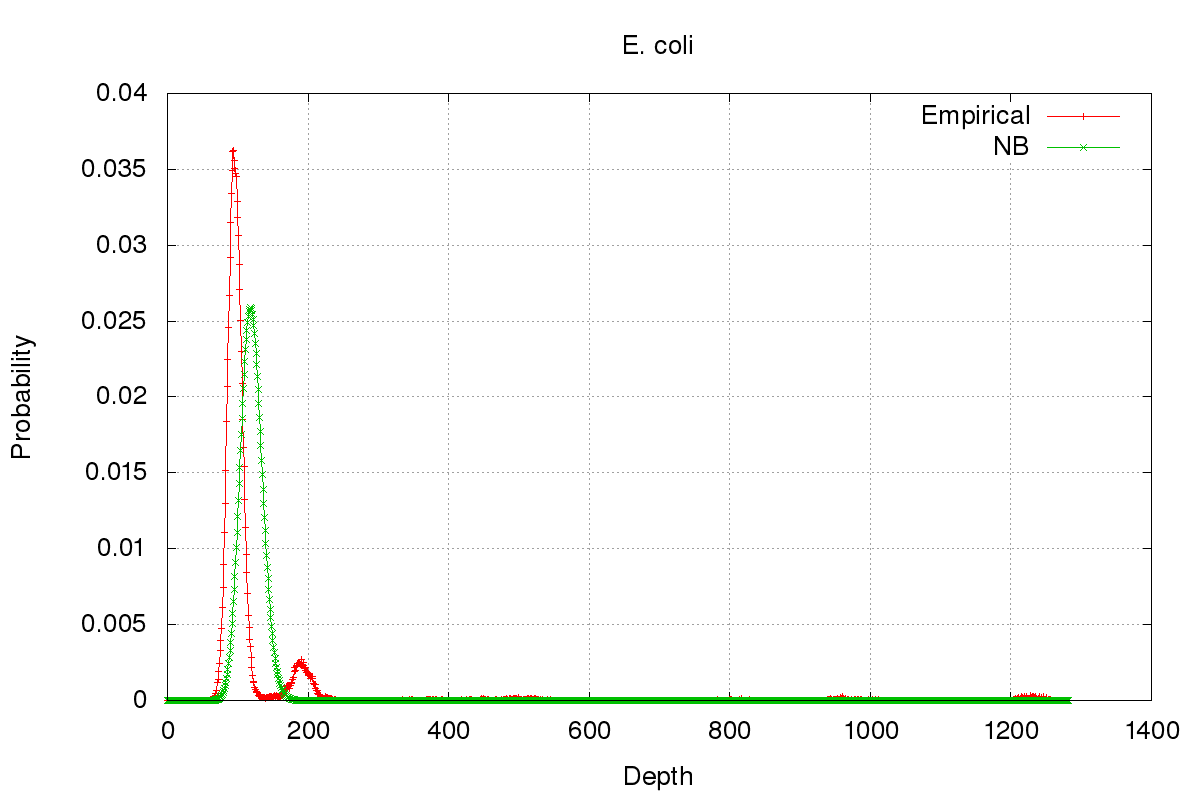
\includegraphics[width=\textwidth]{ecoli_evn.png}
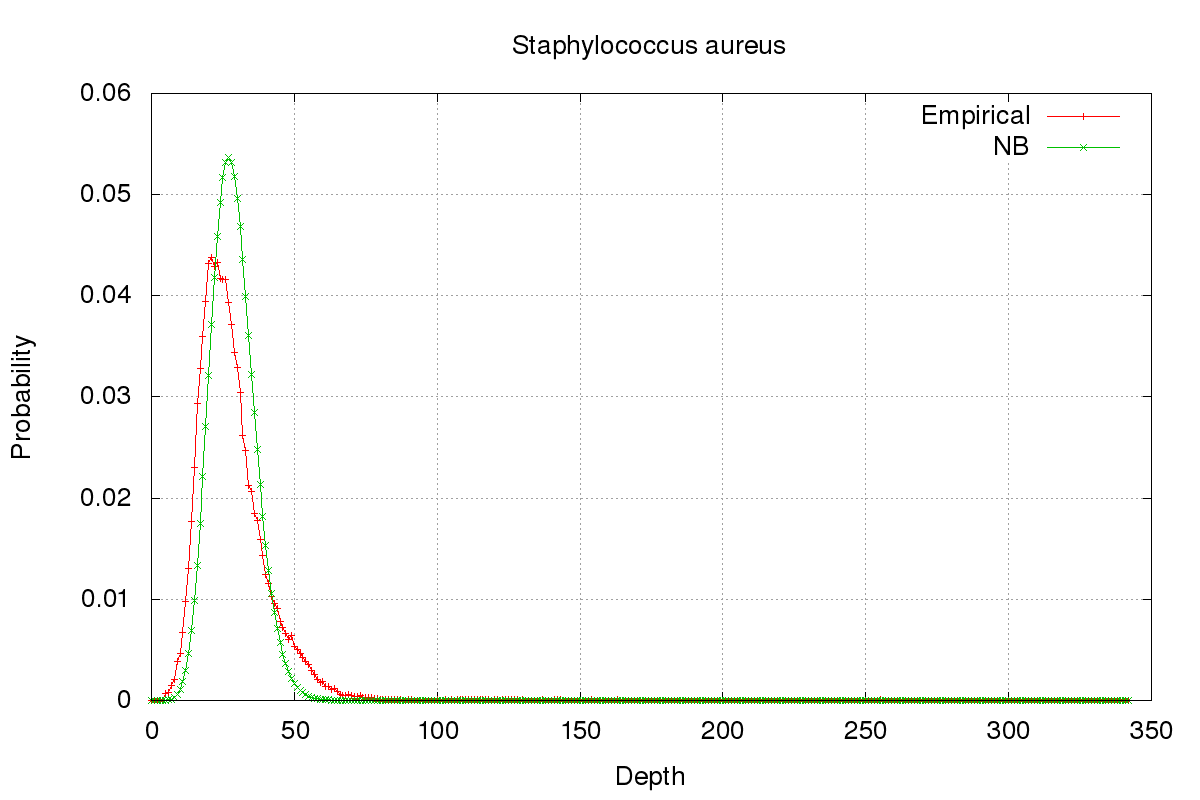
\includegraphics[width=\textwidth]{staphyl_evn.png}
\caption{Графики распределения глубин покрытий для E.coli и для Staphylococcus aureus, посчитанные эмпирически и при помощи отрицательного биномиального распределения.}
\label{fig:NBvsEmp1}
\end{figure}

\begin{figure}[H]
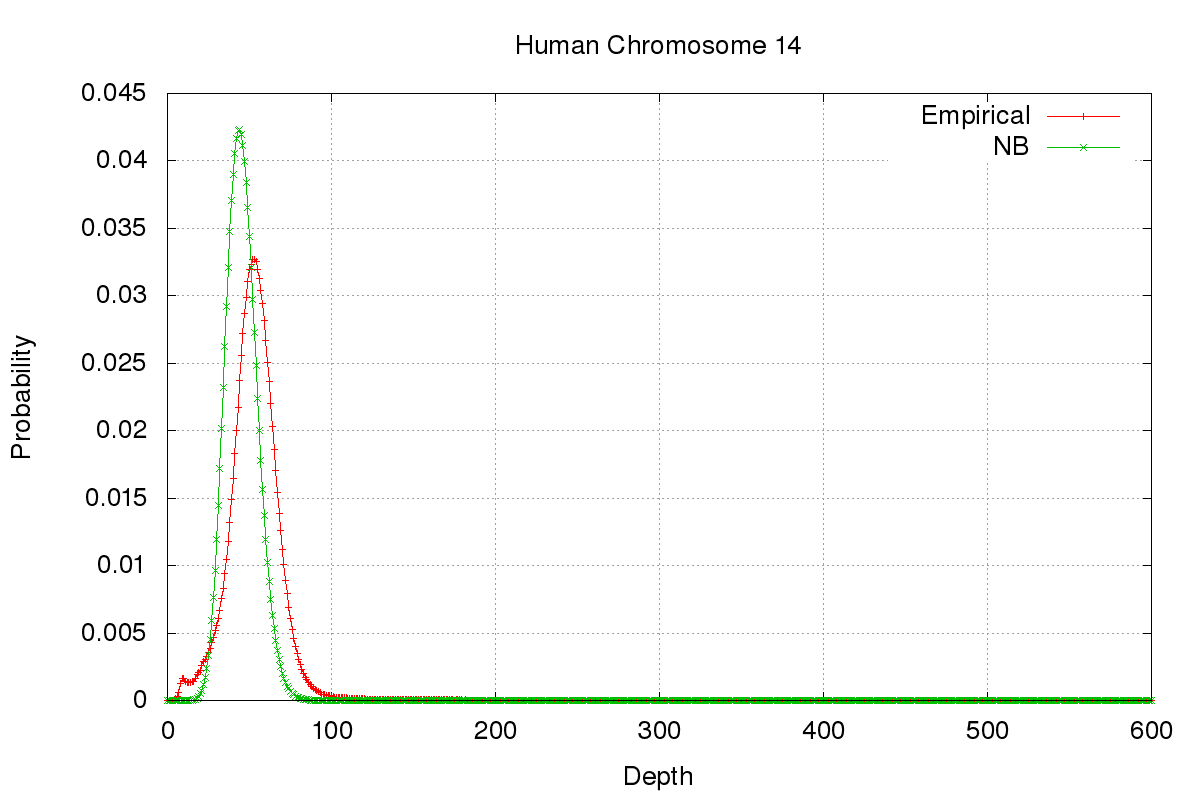
\includegraphics[width=\textwidth]{14cr_evn.png}
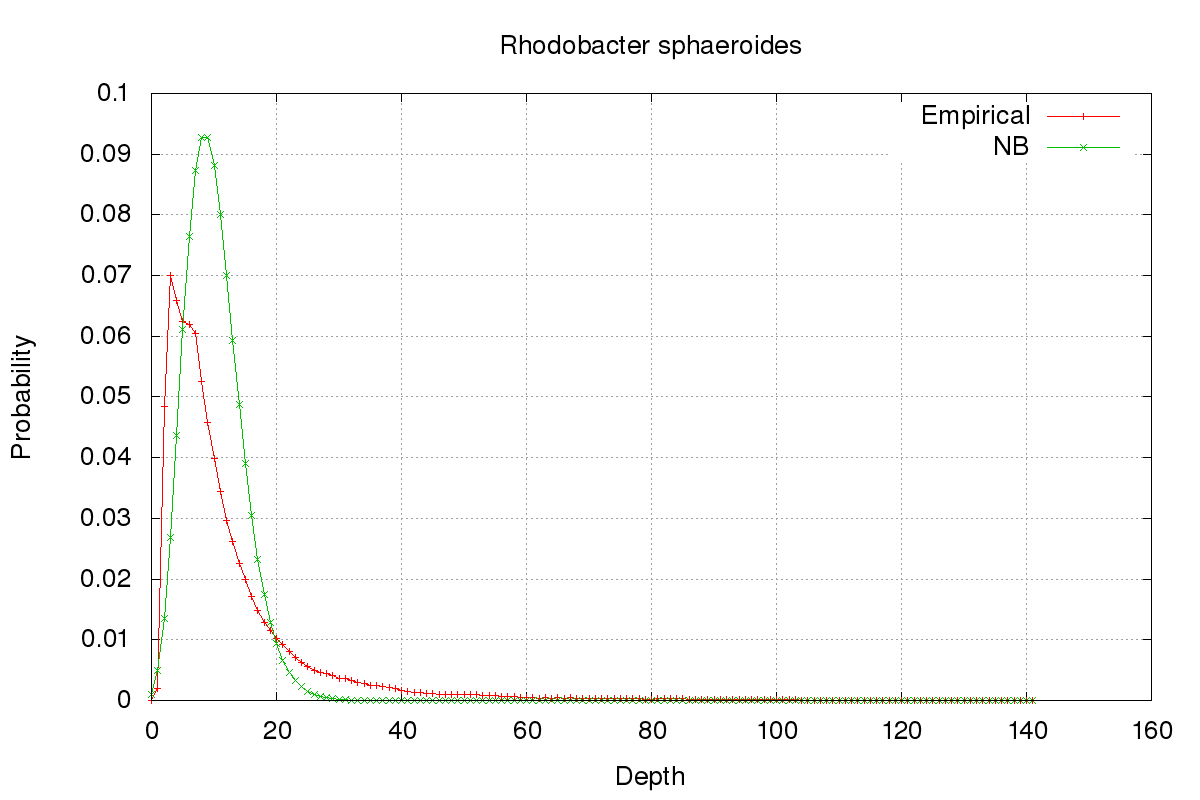
\includegraphics[width=\textwidth]{rhodo_evn.png}
\caption{Графики распределения глубин покрытий для 14-й хромосомы человека и для Rhodobacter sphaeroides, посчитанные эмпирически и при помощи отрицательного биномиального распределения.}
\label{fig:NBvsEmp2}
\end{figure}

Далее было выбрано такое множество GC-контента, которому соответствует максимальное число позиций в сборке, и построены графики сравнения эмпирического и отрицательного биномиального распределения, представленные выше.

Также были приведены статистические тесты, которые показали, что реальное распределение (эмпирическое) не соответствует теоретическому (отрицательному биномиальному). В частности на Staphylococcus aureus $p$-value после $\chi^2$ теста было равно $2\times 10^{-5}$ (за $p=1$ бралась нулевая гипотеза). Приближение на основе принципа максимального правдоподобия также показало отрицательный результат: логарифм вероятности того, что эмпирическое распределение соответствует отрицательному биномиальному $\approx-5$.

\section{Оценка $P_{depth}$}
\subsection{Общая идея}
Предпринимались попытки приближения различными распределениями и комбинациями распределений, однако они не принесли результатов. $p$-value и логарифм вероятности соответствия двух распределений друг другу, описанный выше, либо не удавалось значительно улучшить, либо в случае видимого улучшения на сборке  одного организма метод не работал на сборках других организмов.

В связи с этим для оценки глубины покрытия в каждой позиции в данной работе предлагается использовать эмпирическое распределение. Оно заведомо точнее отрицательного биномиального, поскольку учитывает реальное распределение при заданном наборе чтений.

\subsection{Выбор GC-контента}
Аналогично ALE будем выделять 100 множеств GC-контентов: 0-1, 1-2 ... 99-100\%. Такой выбор связан с тем, у современных секвенаторов Illumina и Ion Torrent средняя длина чтений около 100 нуклеотидов. Были проведены опыты с разбиением на меньшее и большее число множеств. В первом случае существенно падает точность оценки, во втором сильно возрастает время работы оценщика, при этом значительного выигрыша в точности нет.

\subsection{Учёт ошибок}
Эксперименты показали, что в большинстве случаев, нуклеотиды, не покрытые чтениями, являются ошибками сборки геномной последовательности, поэтому предлагается при подсчёте эмпирического рапределения не учитывать позиции в геноме с нулевыми глубинами покрытия. Эффективность такого подхода будет рассмотрена в следующей главе.

\subsection{Анализ производительности}
В отличие от ALE, метод не требует предварительного вычисления средней глубины покрытия для заданного отрезка GC-контента $\mu_{depth}(X_i)$. Для хранения вероятностей глубин в каждой позиции требуется таблица $T$ размером $100\times maxdepth$, где $maxdepth$ -- это максимальное значение глубины покрытия в данной сборке. Нахождение вероятности производится производится обращением к соответствующей ячейке таблицы $T[gc_i][depth_i]$, где $depth_i$ и $gc_i$ -- это соответственно глубина в позиции $i$ и множество, к которому принадлежит GC-контент в позиции $i$.

\section{Выводы к главе 2}